\documentclass{article}
\renewcommand{\thesection}{\Roman{section}} 
\renewcommand{\thesubsection}{\thesection.\Roman{subsection}}
\usepackage{graphicx}
\graphicspath{ {images/} }

\begin{document}

\title{Simulation Study: Classification Performance of Random Forest vs Logistic Regression}
\author{Jacob Brionez, Kaitlin Kirasich, Bivin Sadler, Trace Smith}
\date{\today}

\begin{document}
\maketitle

\begin{abstract} 
Classification and regression performance of statistical based learning algorithms has been widely studied for certain types of data or applications. In supervised learning, the objective of the learning algorithm is to learn a set of parameter estimates such that the loss function is minimized by deploying optimization techniques. Numerous machine learning algorithms currently exist that are utilized for predictive analytics in various domains such as ensemble learners, support vector machines, and neural networks. Selecting a learning algorithm to implement for a particular application on the basis of performance still remains an ad-hoc process using fundamental benchmarks such as evaluating a classifier’s overall loss function, area under the curve (AUC) score, specificity, and sensitivity values. The basis of this work is to present a methodology for evaluating and recommending machine learning classifiers for various simulated data structures benchmarked by retention rate of statistically significant explanatory variables and classification report summary statistics.
\end{abstract}

\section{Introduction}
The success of machine learning models is attributed to identifying predictor variables that best approximates the functional relationship between the input features and the response variable. It is well known that irrelevant features included in a dataset during the training process can lead to rising computational complexity in addition to overfitting, which can present misleading performance metrics as the model will not generalize to the out-of-sample dataset. This work is a proxy for assisting a Data Scientist in deciphering which machine learning model to deploy for a variety of simulated dataset types. This study consists of investigating the performance between Logistic Regression and Random Forest Models for datasets comprised of explanatory variables with varying degrees of correlation in addition to a series of noisy variables which pose no direct relationship with the response. This interactive tool will allow users the flexibility to simulate training datasets such as having a defined number of predictor variables, both large or small, with a specified number of observations. Given the simulated dataset output, the learning algorithm that minimizes the Type I error, failure to reject noise variables by utilizing forward, backward, or stepwise selection criteria, and yields the highest prediction accuracy and AUC score will be proposed algorithm of choice. An analytical tool, developed in R Shiny, will be utilized for simulating a particular data structure that resembles a real-world dataset in order to draw inferences as to which model performs better under certain scenarios and yields the highest precision and accuracy on feature retention rate. For instance, one particular question examines whether Logistic Regression or Random Forest achieves a better performance metric with multiple covariates simulated with various sample sizes. While developing the model recommendation pipeline outlined in this work can be expanded beyond Logistic Regression and Random Forest models, the concept is aimed at providing Data Scientists the tools necessary to evaluate the expected model performance on simulated data before selecting a model to deploy in a real-world application.


\section{Problem}

Within the past few years, the use of predictive analytics has become more prevalent in everyday decision making across many industries.  This is because data is becoming easier to collect and cheaper to store. Picking the best algorithm for a model in predictive analytics is often a challenging task for data scientists.  As with most problems, when it comes to picking between two models, in our case random forest and logistic regression, the answer is, “it depends”.  We have investigated the conditions in which one model performs classification tasks better than another.  We have run conditions of varying ratios of explanatory to noise variables, multiple levels of variance, and increments of sample sizes and simulation iterations.  To compare models as “better” than another, we have looked at misclassification rates, AUC, and type 1 and type 2 errors.

There are numerous studies that compare the random forest and logistic regression algorithms, but we found that most research experiments used either a single dataset or multiple datasets from the same source.  In these scenarios, sometimes logistic regression performed better and sometime random forest performed better.  For example, we found an experiment using several neuropsychological tests to predict dementia reported that, with respect to specificity and overall classification accuracy, random forests and linear discriminant analysis rank first among all the classifiers including logistic regression (Guerreiro, 2011).  Contrastingly, in another article analyzing Twitter tweets surrounding the 2016 United States election, it was found that when PCA is applied to tweets, logistic regression provides better results than random forest (Beğenilmiş, 2017).  These types of data and data sources are drastically different from each other and each algorithm performs differently due to the type of data it was using to try to classify. 

\par
Criteria for identifying significant input features in a model varies between domains and datasets at hand. Automated feature selection has widely been studied, ranging from computer vision, classification, and regression types of problems. Zoran et al proposed a purposeful selection of covariates algorithm that automates feature selection by iteratively refitting the model by either adding or removing variables to verify if the model contains statistically significant predictors or confounders with a maximum p-value of 0.25 (Zoran, 2008). Traditionally, the significance threshold is 0.05; although there is only a 5\% chance of a Type I error, variables of importance could be misclassified. In this simulation study, the purposeful selection method evaluates significance at the 0.10 level and if the parameter estimate value alters 20\% compared to the full model, then there is evidence the excluded variable was of importance and is therefore added back to the model (Zoran, 2008). The novel method was applied on two different simulated datasets and was compared with stepwise, forward, and backward selection as a benchmark for the conclusion.
 
\par
Logistic Regression was the model of choice for the two simulation experiments performed by Zoran et al, consisting of six total explanatory variables and six different sample sizes. The first study consisted of only three significant variables of equal parameter estimates and three non-significant predictors. Secondly, the simulation was altered slightly to contain two significant variables, one confounder which is dependent on X1, and three non-significant variables with parameter estimate of zero, respectively. For both simulation cases, the average retention rate for 1000 iterations correctly identified variables increased with respect to an increase in sample size (Zoran, 2008). 

\par
Additionally, TPOT is a recently developed tool built in Python and optimizes machine learning pipelines via genetic programming with the goal of maximizing classification accuracy on any supervised classification problems (Olsen, 2016). Similar to what a content management system is to a website where anyone who has no knowledge of web development can edit a website, TPOT does the same for machine learning.  The tool takes in a dataset and picks out the best features to generate an optimized model for prediction and classification (Olsen, 2016).  The other feature engineering tool we found is called One Button Machine, or OneBM, which automates the extraction of useful features from relational databases (Lam, 2017).  We hope to take our simulated data and run it through either TPOT or OneBM and see how well their feature engineering works and if it helps either random forest or logistic regression performance. 

\section{Machine Learning Models}

\subsection{Random Forest}

Random forest is the first regression and classification algorithm we will use for our project.  Random forest is made up of multiple learning algorithms which we call decisions trees.  These decision trees work together, in ensemble, to classify or predict.  A decision tree or machine learning algorithm by itself is prone to building a model that tends to over-fit the noise in the training set leading to results with a high variance.  This means that the model could accurately predict the same data it was trained on but may not work on datasets without the exact same patterns and variations.  Random forest solves this overfitting of data by averaging multiple decision trees trained on different parts of the training set. The idea is the predictions of a single decision tree may be sensitive to noise, but the average of many trees is not which lowers the variance thus improves accuracy.  However, this idea will only hold as long as the trees are not correlated which is why we train on multiple parts of the training set.

To average and combine the decision trees, random forest uses bootstrap aggregating, or bagging.  Bagging in random forests works by continually sampling a random subset of features to train our decision trees on.  After training our trees, we make a prediction based on the average of each individual decision tree’s prediction.  Bagging leads to better model performance because it decreases the variance of the model, without increasing the bias.  As we build our forest, random forest generates an internal unbiased estimate of the generalization error.

Random forest can also be used to return estimates of what variables are important in the classification by collecting out of bag measurements which is the error for each data point recorded and averaged over the forest.  

\subsection{Logistic Regression}

Linear models are composed of one or multiple independent variables that describes a relationship to a dependent response variable. Mapping qualitative or quantitative input features to a target variable that is attempted to being predicted such as financial, biological, or sociological data is known as supervised learning in machine learning terminology if the labels are known.  One of the most common utilized linear statistical models for discriminant analysis is Logistic Regression.

Simplicity and interoperability of Logistic Regression can occasionally lead to outperforming other sophisticated nonlinear models such as ensemble learners or support vector machines. However, in the event the response variable is drawn from a small sample size, then linear regression models become insufficient and performs poorly for binary responses A number of learning algorithms could be applied to modeling binary classification data types, however the focal point of this work is to examine one linear model, logistic regression. 
 
Unlike the response variable for Linear Regression which is quantitative, the target variable for Logistic Regression is the posterior probability of being classified in the ith group of a binary or multi-class response (Hastie, 2009). Logistic Regression makes several assumptions such as independence, responses (logits) at every level of a subpopulation of the explanatory variable are normally distributed, and constant variance between the responses and all values of the explanatory variable. Intuitively, a transformation to the response variable is applied to yield a continuous probability distribution over the output classes bounded between 0 and 1; this transformation is called to “logistic” or “sigmoid” function where ‘z’ corresponds to log odds divided by the logit (Ng, 2008).

\begin{figure}[h]
\centering
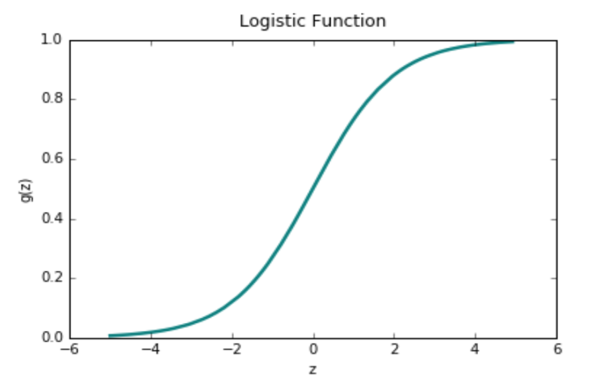
\includegraphics[scale=1.0]{sigmoid.png}
\caption{Log of Odds Function}
\end{figure}

For a binary response, the Logistic Regression model can be expressed by summing over the linear combinations of input features and a corresponding weight plus a bias terms for each instance as shown in Eq.3 and Eq.4.

The objective is to find a set of weights such that the negative log likelihood is minimized over the defined training set using optimization techniques such as gradient descent or stochastic gradient descent [3]. Minimizing the negative log likelihood also means maximizing the likelihood or probability the parameter estimate pi of selecting the correct class. The loss function that measures the difference between the ground truth label and the predicted class label is referred to as the cross-entropy (Eq.5). If the prediction is very close to the ground truth label, the loss value will be low. Alternatively, if the prediction is far from the true label, the resulting log loss will be higher.


\section{Criteria for Comparison}

The criteria we use to compare a machine learning algorithm’s model selection performance are type 1 errors, type 2 errors, and AIC.  When comparing the machine learning model’s accuracy we use the misclassification rates and AUC.  

Type 1 errors are defined as a false positive finding.  We use this when looking at what variables each model selects.  A type 1 error is when a machine learning algorithm finds a model that includes noise variables thinking it is an explanatory variable.  Type 2 errors are the false negative findings that occur when our machine learning algorithm chooses a model that leaves out a true explanatory variable.

The Akaike information criterion, or AIC, is an estimator of quality in model selection.  We use this when comparing the same type of model under different conditions.  It comes from information theory as estimate of the relative information lost when a given model is used to represent the process that generated the data.  It cannot define the quality of one model, but it can define the quality relative to another model.

After selecting a model from each algorithm and training it, we compare models using misclassification rates.  We look at the true positive rate (sensitivity), true negative rate (specificity), false positive rate, and false negative rate.  True positive rate and sensitivity are calculated as the portion of positives or successes that are correctly identified.  False positive rate is the portion that was incorrectly identified as positive or success but is actually negative.  True negative rate and specificity are defined as the portion of negatives that are correctly identified.  The false negative rate would be the portion of incorrectly identified negatives.  Depending on your application, you may care about incorrectly classifying a positive more than incorrectly classifying a negative.  For example, when dealing with anything medical or health related, one is likely more focused on correctly identifying a positive and minimizing the false negative rate.  When dealing with automated event or airport security, it may be okay to have a higher false negative rate because it may be cheap and non-life threatening to confirm the automated alert.

These data points can be graphically represented using the receiver operating characteristic curve or ROC curve.  The ROC curve is a graph with the x axis from 0 to 1 of the false positive rate, and the y axis from 0 to 1 of the true positive rate at various threshold settings.  A perfect predictor would have a false positive rate of 0 and a true positive rate of 1.  When graphed over a series of thresholds, we would want to look at the area under the curve, or AUC.  The higher the AUC, the better our model performs.  

\section{Results}


\section{Ethics}
We are building a tool to generate the data in an effort to evaluate and compare the logistic regression and random forest models.  Since all data will be simulated via our tool we do not anticipate any ethical concerns. For future work, we may allow users to upload their own dataset to our tool to run an evaluation.  In this case, we will not store or publish any of the users’ data inside the app.  We will also notify the users that our tool should be used for education purposes only.  Because we are not storing any data, we will not run a security scan on our application but we will use best practices to avoid any known vulnerabilities. If any issues are reported we will also notify users of potential deficiencies as well as correct these deficiencies if possible.

\section{Conclusion}

The application we built provides users with a clean and simple interface to compare logistic regression and random forest models over a variety of different types of data sets to facilitate data scientists in choosing the best model for their needs.  After using our own tool to compare models, we found that random forest works best for data where …


\section{Reference}

Guerreiro, Manuela; Maroco, João; de Mendonça, Alexandre; Rodrigues, Ana; Santana, Isabel; Silva, Dina. Data mining methods in the prediction of Dementia: A real-data comparison of the accuracy, sensitivity and specificity of linear discriminant analysis, logistic regression, neural networks, support vector machines, classification trees and random forests. BMC Research Notes20114:299. https://doi.org/10.1186/1756-0500-4-299.

Beğenilmiş, Erdem; Üsküdarlı, Suzan.  Organized Behavior Classification of Tweet Sets using Supervised Learning Methods. eprint arXiv:1711.10720. 11/2017.

Thanh Lam, Hoang; Thiebaut, Johann-Michael; Sinn, Mathieu; Chen, Bei; Mai, Tiep; Alkan, Oznur.  One button machine for automating feature engineering in relational databases. eprint arXiv:1706.00327. 06/2017.

Olson, Randal S.; Moore, Jason H.  Identifying and Harnessing the Building Blocks of Machine Learning Pipelines for Sensible Initialization of a Data Science Automation Tool. eprint arXiv:1607.08878. 07/2016. 

Graham Dunn. (2007) Regression Models for Method Comparison Data. Journal of Biopharmaceutical Statistics 17:4, pages 739-756

Hastie, T., Tibshirani, R., Friedman, J. (2009). The elements of statistical learning: data mining, inference and prediction. Springer. 

Andrew Ng. CS229 Lecture Notes. Stanford University. 2012

Zoran Bursac, C Heath Gauss, David Keith Williams, David W Hosmer: Purposeful Selection of Variables in Logistic Regression. Source Code for Biology and Medicine. 2008



\end{document}

